\documentclass[10pt,fleqn]{article} % Default font size and left-justified equations
\usepackage[%
    pdftitle={SLCI : Cinématique du solide},
    pdfauthor={Xavier Pessoles}]{hyperref}

\input{style/new_style}
\input{style/macros_SII}
\usepackage{style/schemabloc}

%\fichetrue
\fichefalse

%\proftrue
\proffalse

%\tdtrue
\tdfalse

\courstrue
%\coursfalse

% -------------------------------------
% Déclaration des titres
% -------------------------------------

\def\discipline{Sciences \\Industrielles de \\ l'Ingénieur}
\def\xxtete{Sciences Industrielles de l'Ingénieur}

\def\classe{PTSI}
\def\xxnumpartie{Partie 2}
\def\xxpartie{Découverte des Systèmes Linéaires Continus et Invariants\\
Analyse, Modélisation, Résolution}

\def\xxnumchapitre{Chapitre 4}
\def\xxchapitre{\hspace{.12cm} Étude des systèmes fondamentaux du premier ordre}

\def\xxposongletx{2}
\def\xxposonglettext{1.45}
\def\xxposonglety{23}
\def\xxonglet{Part. 2 -- Ch. 4}

\def\xxactivite{Cours}
\def\xxauteur{\textsl{Xavier Pessoles}}

\def\xxcompetences{%
\textsl{%
\textbf{Savoirs et compétences :}
\begin{itemize}[label=\ding{112},font=\color{ocre}] 
\item Mod-C2.3 : Modèles canoniques du premier ordre
\begin{itemize}[label=\ding{112},font=\color{ocre}] 
\item Mod-C2-S1 : Identifier le comportement d’un système pour l’assimiler à un modèle canonique, à partir d’une réponse temporelle 
\item Mod-C2-S2 : Établir un modèle de comportement à partir de relevés expérimentaux
\item Mod-C2-S3 : On pourra étudier les systèmes du premier ordre présentant un retard pur
\end{itemize}
\end{itemize}
}}

\def\xxfigures{
\includegraphics[height=3cm]{images/circuit_RC.png} 

\textit{Charge d'un condensateur}

\includegraphics[height=2.5cm]{images/mcc.png} 

\textit{Moteur à courant continu (suivant les hypothèses)}
}%figues de la page de garde
\def\xxpied{%
Partie 2 -- Découverte des SLCI\\
Ch. 4 : Étude des systèmes fondamentaux du premier ordre -- \xxactivite%
}

%---------------------------------------------------------------------------


\begin{document}
\chapterimage{png/Fond_SLCI}
\input{style/new_pagegarde}

%
%
%\begin{obj}
%\textsc{Problématique :}
%\begin{itemize}
%\item Le comportement réel de certains systèmes asservis peut se modéliser par des systèmes dits du premier ordre. Comment modéliser de tels systèmes ?
%%\item Comment modéliser un système complexe multiphysique en utilisant la modélisation en schéma bloc et la modélisation dans le domaine de Laplace ?
%%\item Comment déterminer la fonction de transfert d'un système dans le but de prévoir son comportement ?
%\end{itemize}
%\end{obj}
%
%
%
%\begin{savoir}
%\textbf{Savoirs :}
%\end{savoir}
%
%
%
%%\begin{rem}
%%\textbf{Remarque}
%%
%%Tous les résultats synthétisés dans ce cours ont été démontrés dans le TD intitulé \textit{Analyse théorique des systèmes du premier ordre}.
%%\end{rem}
%
%
%\setlength{\parskip}{0ex plus 0.2ex minus 0ex}
% \renewcommand{\contentsname}{}
% \renewcommand{\baselinestretch}{1}
%
%% \vspace{1cm}
%\textit{Ce document est en évolution permanente. Merci de signaler toutes
%erreurs ou coquilles.}
%
%\tableofcontents
%
% \renewcommand{\baselinestretch}{1.2}
%\setlength{\parskip}{2ex plus 0.5ex minus 0.2ex}


\section{Définition}

Les systèmes du premier ordre sont régis par une équation différentielle de la
forme suivante :
$$
\tau \dfrac{ds(t)}{dt}+s(t) = Ke(t)
$$


\begin{minipage}[c]{.6\linewidth}
\begin{defi}
Dans le domaine de Laplace, la fonction de transfert de ce système est donc
donnée par :

$$
H(p)=\dfrac{S(p)}{E(p)} = \dfrac{K}{1+\tau p}
$$

On note :
\begin{itemize}
 \item $\tau$ la constante de temps ($\tau>0$);
\item $K$ le gain statique du système ($K>0$).
\end{itemize}
\end{defi}
\end{minipage}\hfill
\begin{minipage}[c]{.35\linewidth}
Schéma-bloc d'un système du premier ordre :

\begin{center}
\begin{tikzpicture}
\sbEntree{E}
\sbBloc[5]{B1}{$H(p)=\dfrac{K}{1+\tau p}$}{E}
\sbSortie[5]{S}{B1}
\sbRelier[$E(p)$]{E}{B1}
\sbRelier[$S(p)$]{B1}{S}
\end{tikzpicture}
\end{center}
\end{minipage}

\section{Caractéristiques de la réponse impulsionnelle}
Par définition on rappelle que la réponse impulsionnelle correspond à la courbe de réponse du système sollicité par une fonction de Dirac.


\begin{minipage}[c]{.4\linewidth}
\begin{center}
\begin{tabular}{p{0.6\textwidth}l}
%\hline
%& \\
Réponse temporelle : & $s(t)=\dfrac{K}{\tau}e^{-\dfrac{t}{\tau}}$ \\
& \\
Valeur initiale : & $s(0)=\dfrac{K}{\tau}$ \\
& \\
Valeur finale : & $\lim\limits_{t\to +\infty }s(t)=0$\\
& \\
Équation de la tangente à l'origine : & $\Delta(t)=\dfrac{K}{\tau}-\dfrac{K}{\tau^2}t$\\
%& \\
%\hline
\end{tabular}
\end{center}
\end{minipage} \hfill
\begin{minipage}[c]{.55\linewidth}
\begin{center}
 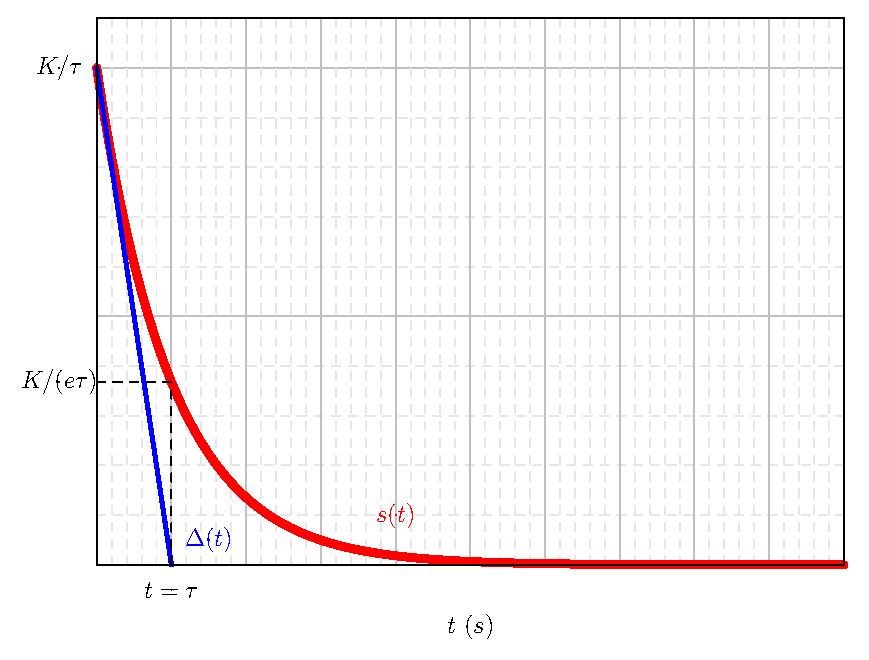
\includegraphics[width=.95\textwidth]{images/ordre1_dirac}
\end{center}
\end{minipage}




\begin{demo}
\textit{Éléments de démonstration}

Dans le cas d'une réponse impulsionnelle, l'entrée est un Dirac : on a donc $E(p)=1$. 

En conséquence, 
$$
S(p)=E(p)\cdot H(p) = \dfrac{K}{1+\tau p}
$$

La transformée de Laplace inverse permet de conclure directement que :
$$
\forall t>0 \quad s(t)=\dfrac{K}{\tau}e^{-\dfrac{t}{\tau}}
$$

\end{demo}


\section{Caractéristiques de la réponse indicielle}
Par définition on rappelle que la réponse indicielle correspond à la courbe de réponse du système sollicité par une fonction échelon d'amplitude $E_0$ : $\forall t>0,\quad  e(t)=E_0 $.



%\subsection*{Caractéristiques de la réponse temporelle}
\begin{minipage}[c]{.4\linewidth}
\begin{center}
\begin{tabular}{p{.4\textwidth}l}
%\hline
Réponse temporelle : & $
s(t)=KE_0 \left( 1-e^{-\dfrac{t}{\tau}}\right)u(t)
$ \\
& \\
Valeur initiale : & $s(0)=0$ \\
& \\
Valeur finale : & $\lim\limits_{t\to +\infty }s(t)=K\cdot E_0$\\
& \\
Équation de la tangente à l'origine : & $\Delta(t)= \dfrac{KE_0}{\tau} t$\\
\end{tabular}
\end{center}
\end{minipage} \hfill
\begin{minipage}[c]{.54\linewidth}
\begin{center}
 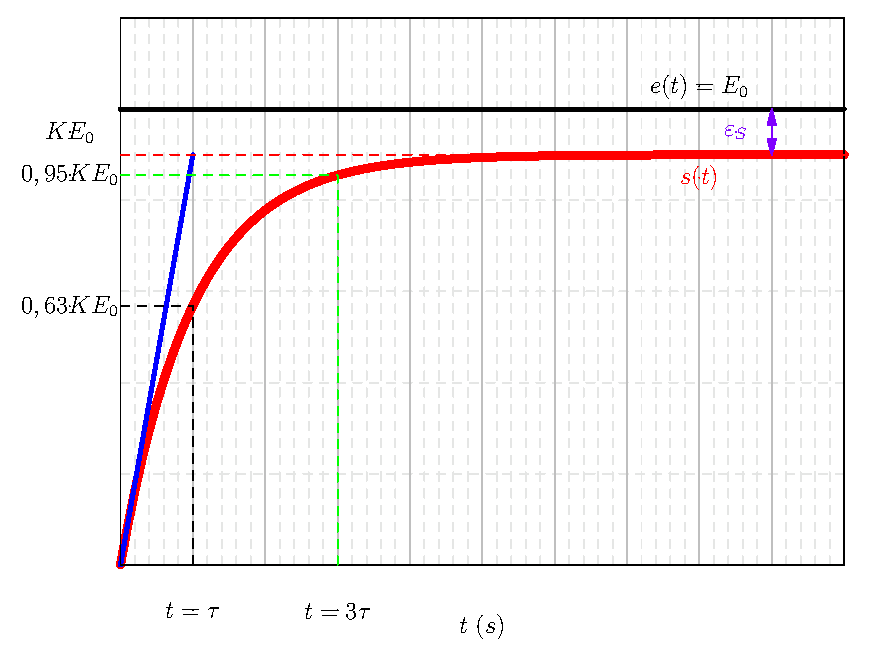
\includegraphics[width=\textwidth]{images/ordre1_echelon}
\end{center}
\end{minipage}



\subsection*{Caractéristiques remarquables de la réponse indicielle}


\begin{rem}
L'écart statique d'un système du premier ordre répondant à une entrée
indicielle est nul si le gain $K$ est égal à 1.
\end{rem}


\begin{resultat}
Pour $t=\tau$, 
$$
s(\tau)=KE_0 (1-e)\simeq 0,63 KE_0
$$

Lorsque $t=\tau$ la sortie a donc atteint 63\% de la valeur finale.
\end{resultat}

\begin{resultat}
On note $t_r$ le temps de réponse à 5\%.

$$ t_r = - \ln \left(0,05\right) \tau \simeq 3\tau
$$

\end{resultat}



\begin{demo}
\textit{Éléments de démonstration}


Dans le cas d'une réponse indicielle, l'entrée est un échelon d'amplitude $E_0$, on a donc $E(p)=\dfrac{E_0}{p}$. 

En conséquence, 
$$
S(p)=E(p)\cdot H(p) = \dfrac{E_0}{p} \cdot \dfrac{K}{1+\tau p}
$$

$S(p)$ se décompose en éléments simples de la façon suivante :
$$
S(p)= \dfrac{\alpha}{p} + \dfrac{\beta}{1+\tau p} = \dfrac{E_0 K}{p}- \dfrac{E_0 K \tau}{1+\tau p}
$$

La transformée de Laplace inverse permet de conclure que :
$$
\forall t>0  \quad s(t)=KE_0 \left( 1-e^{-\dfrac{t}{\tau}}\right)
$$

\end{demo}

\section{Caractéristiques de la réponse à une rampe}
On sollicite un système du premier ordre avec une rampe de pente $A$.
On a $e(t)=Atu(t)$ dans le domaine temporel et $E(p)=\dfrac{A}{p^2}$ dans le domaine de Laplace.



\noindent\begin{minipage}[c]{.4\linewidth}
\begin{center}
\begin{tabular}{ll}
%\hline
Réponse temporelle : & 
$s(t)=AK\left( t-\tau+\tau e^{-\dfrac{t}{\tau}}
\right) u(t)$  \\
& \\
Valeur initiale : & $s(0)=0$ \\
& \\
Valeur finale : & $\lim\limits_{t\to +\infty = 0}s(t)=+\infty $\\
& \\
Coefficient directeur & \\
de l'asymptote en $+\infty $ :& $AK$\\
& \\
Erreur dynamique : & $AK\tau$\\
\end{tabular}
\end{center}
\end{minipage}\hfill
\begin{minipage}[c]{.48\linewidth}
\begin{center}
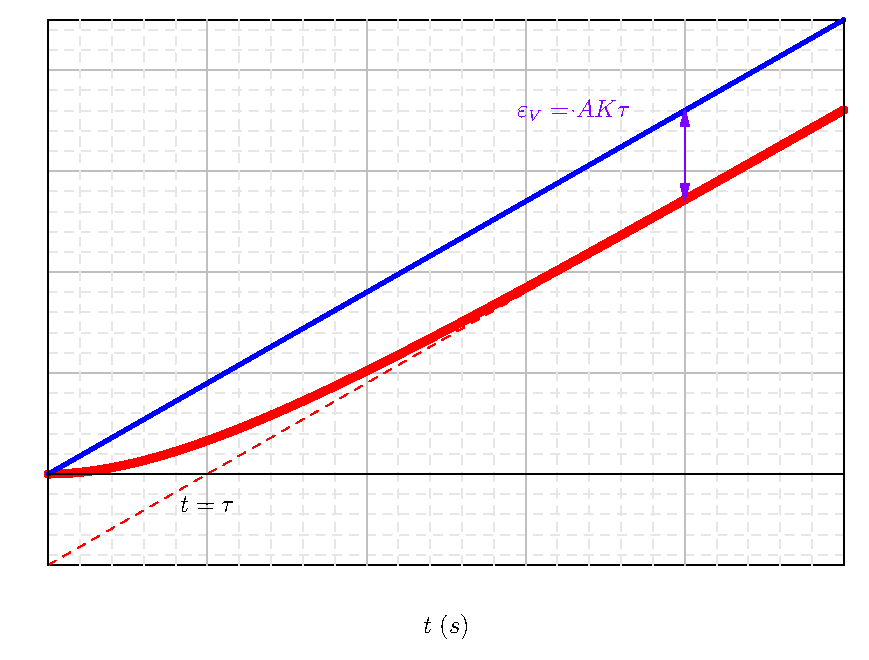
\includegraphics[width=\textwidth]{images/ordre1_rampe}
\end{center}
\end{minipage}



\end{document}

\section{Exemples}
Les courbes suivantes représentent la réponse indicielle à un échelon.
Identifier les systèmes à partir des courbes.
Les constantes de temps seront données à partir des 3 méthodes vues en cours.

\begin{center}
%  \includegraphics[width=.75\textwidth]{eps/ordre1_echelon_exo1-1}
\end{center}

\begin{center}
%  \includegraphics[width=.75\textwidth]{eps/ordre1_echelon_exo2-1}
\end{center}
\end{document}
